% ================= Appendix A =================
\chapter{Raw Dataset}
\label{app:A.1}
 \label{fig:samplerawdatas}
\begin{figure}[H]
    \centering
    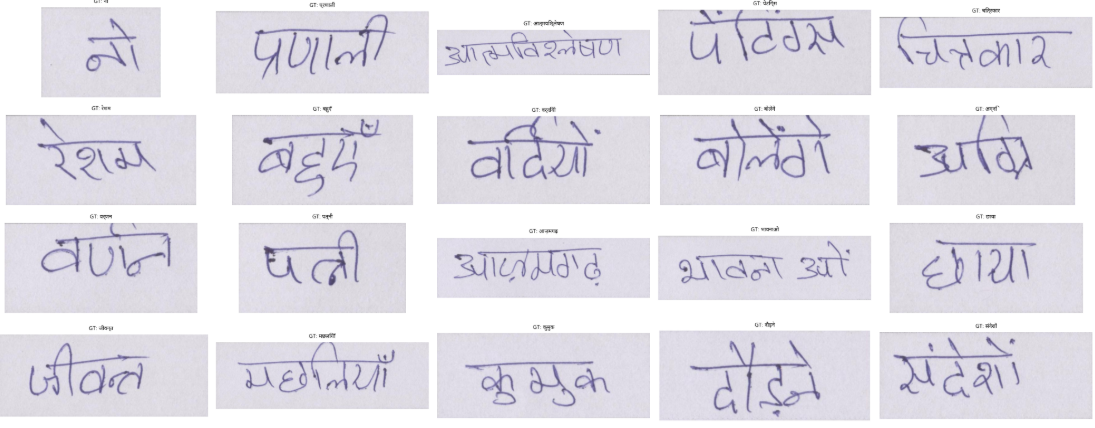
\includegraphics[width=0.7\textwidth]{img/rawdata.png}
    \caption{Sample raw dataset}
   
\end{figure}


% ================= Appendix B =================
\chapter{Image Pre-processing Pipeline Details}
\label{app:preprocessing}
\section{Grayscale Conversion and Denoising}
\label{app:B1}
\begin{figure}[H]
    \centering
    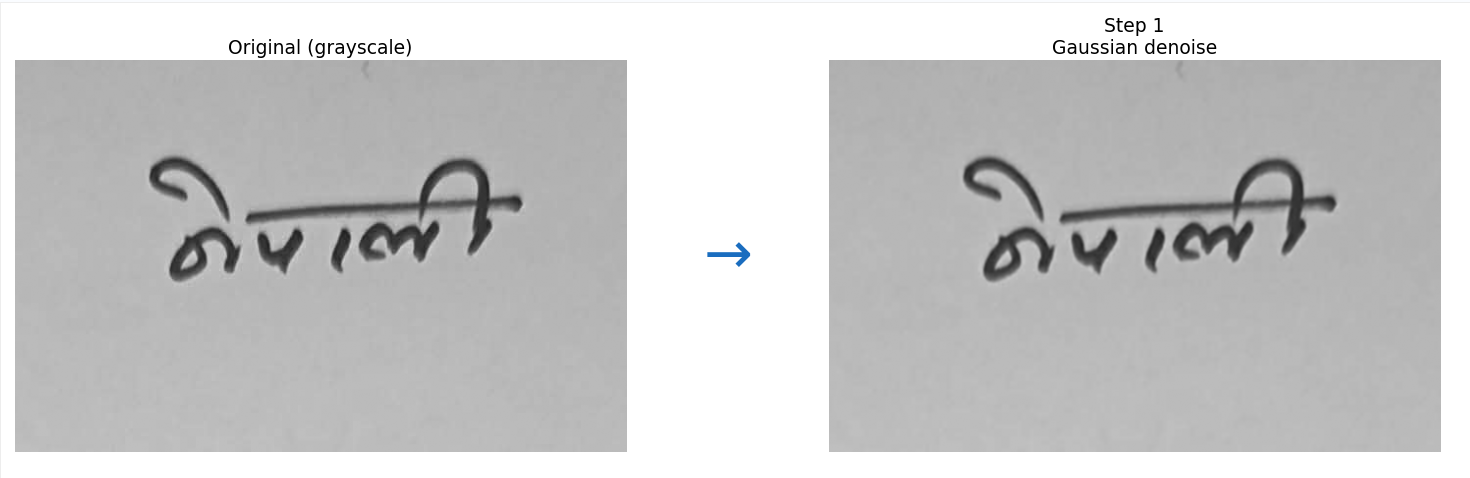
\includegraphics[width=0.7\textwidth]{img/step1_grayscale_denoise.png}
    \caption{Grayscale conversion with $3 \times 3$ Gaussian blur}
\end{figure}

\section{Adaptive Binarisation}
\label{app:B2}
\begin{figure}[H]
    \centering
    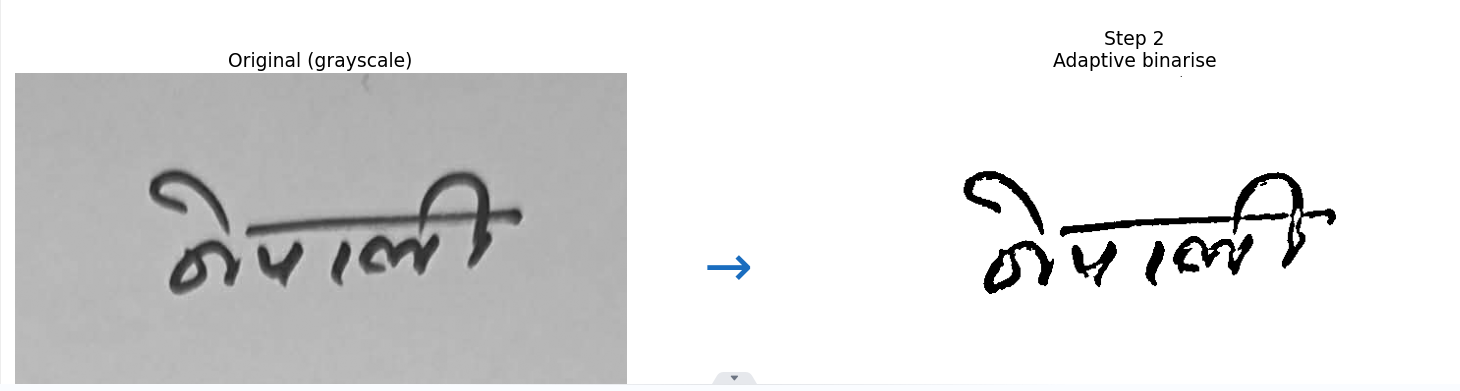
\includegraphics[width=0.7\textwidth]{img/step2_adaptive_binarization.png}
    \caption{Adaptive Gaussian threshold}
\end{figure}

\section{Morphological Closing}
\label{app:B3}
\begin{figure}[H]
    \centering
    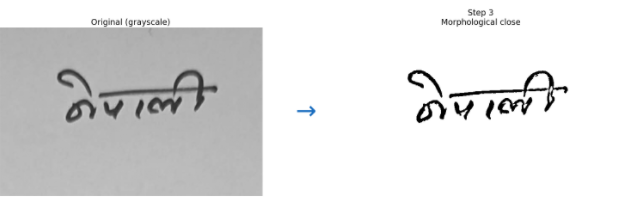
\includegraphics[width=0.7\textwidth]{img/step3_morphological_closing.png}
    \caption{Closing operation}
\end{figure}

\section{Deskewing}
\label{app:B4}
\begin{figure}[H]
    \centering
    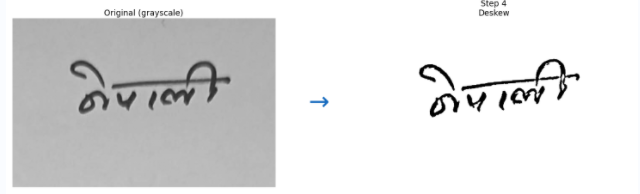
\includegraphics[width=0.7\textwidth]{img/step4_deskewing.png}
    \caption{Skew correction}
\end{figure}

\section{Tight Cropping}
\label{app:B5}
\begin{figure}[H]
    \centering
    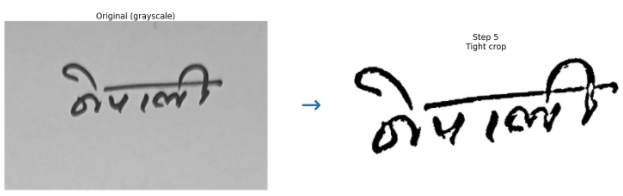
\includegraphics[width=0.7\textwidth]{img/step5_tight_cropping.png}
    \caption{Bounding box cropping}
\end{figure}

\section{Letterbox Padding and Resize}
\label{app:B6}
\begin{figure}[H]
    \centering
    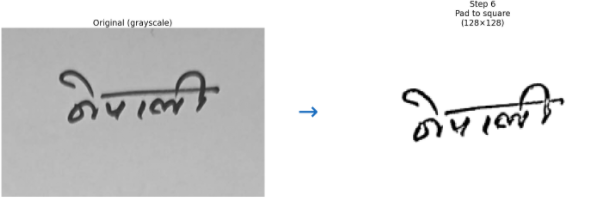
\includegraphics[width=0.7\textwidth]{img/step6_letterbox_padding.png}
    \caption{Resizing to $128 \times 128$}
\end{figure}

\section{RGB Conversion and Normalisation}
\label{app:B7}
\begin{figure}[H]
    \centering
    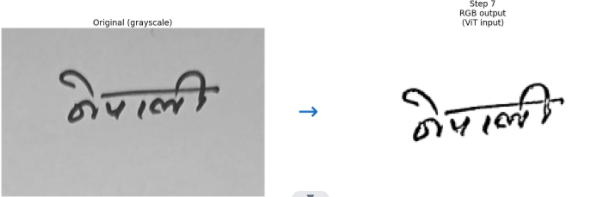
\includegraphics[width=0.7\textwidth]{img/step7_rgb_normalization.png}
    \caption{RGB conversion and normalization}
\end{figure}


% ================= Appendix C =================
\chapter{User Interface Screenshots}
\label{app:C1}

\section{Main Interface}
\begin{figure}[H]
    \centering
    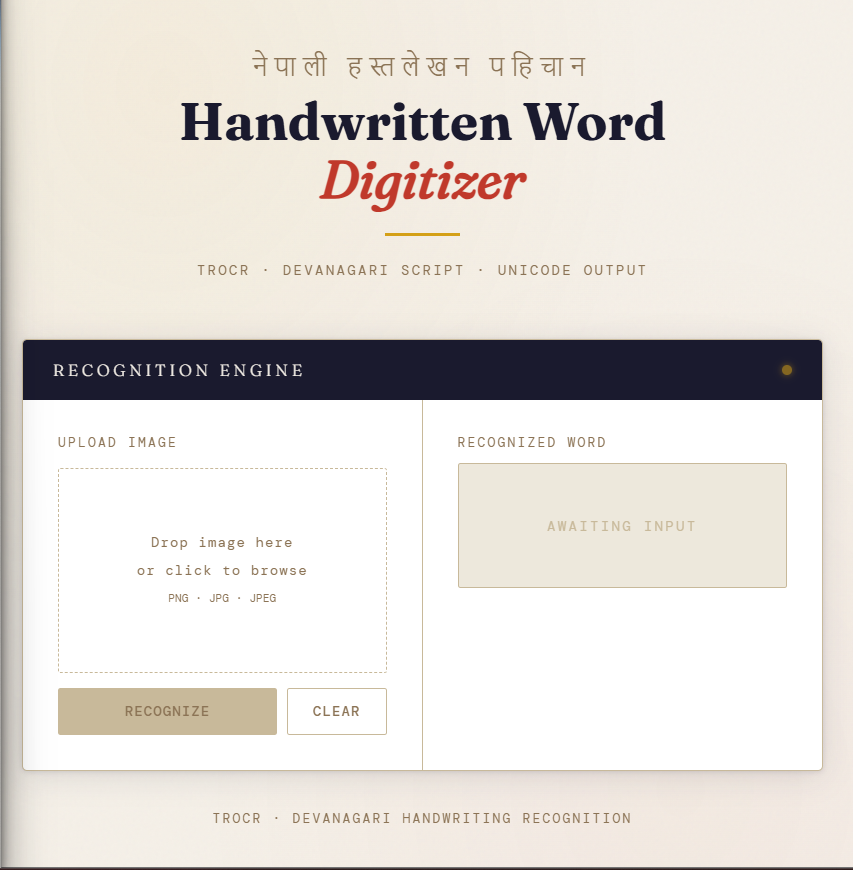
\includegraphics[width=0.72\textwidth]{img/screenshot_main.png}
    \caption{Main interface}
\end{figure}

\section{Recognized Word}
\begin{figure}[H]
    \centering
    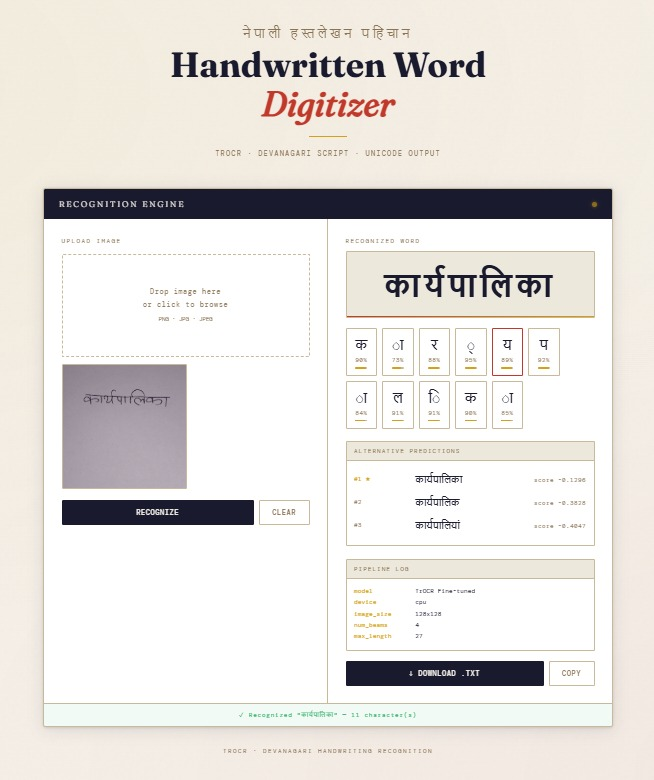
\includegraphics[width=0.75\textwidth]{img/output1.jpeg}
\end{figure}

\begin{figure}[H]
    \centering
    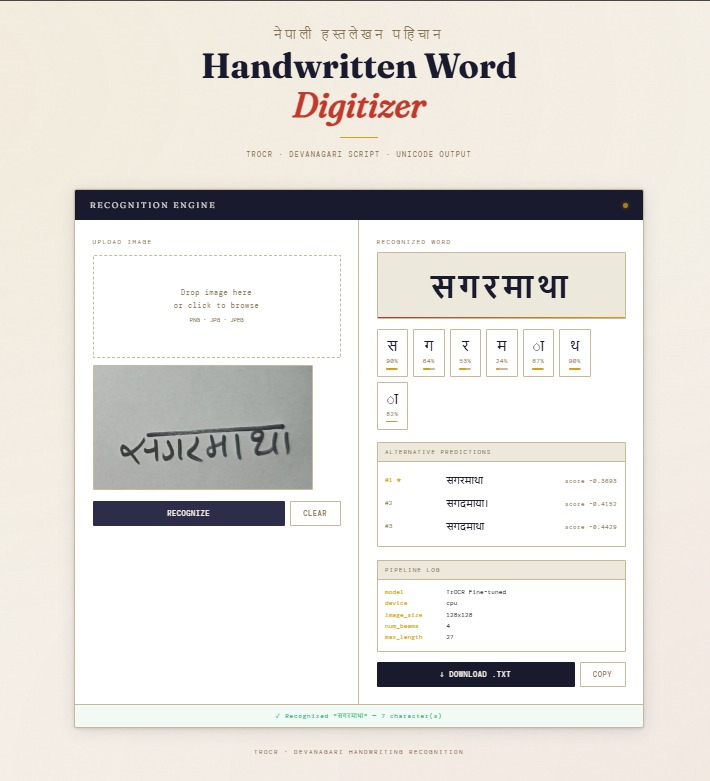
\includegraphics[width=0.75\textwidth]{img/output2.jpeg}
    \caption{Generated word}
\end{figure}